\documentclass[12pt,letterpaper]{article}
\usepackage[utf8]{inputenc}
\usepackage{graphicx}
\usepackage{tikz}
\usetikzlibrary{arrows,positioning}  %Agregamos las bibliotecas arrows y positioning de tikz, para soportar el uso de flechas y el control del posicionamiento entre los nodos 
%Definimos el tipo de flecha estándar
\tikzset{
	>=stealth',
}
\usepackage[hidelinks]{hyperref}
\author{Curso de \LaTeX}
\title{Representación de redes utilizando graficos con TikZ}
\begin{document}
\maketitle

Una red es la representación de un sistema complejo en un conjunto de elementos conectados entre sí por relaciones. Entre sus aplicaciones en las ciencias marinas tenemos:

\textbf{Red trófica}

\begin{tikzpicture}[node distance=3cm, auto]
\node (ave) {\includegraphics[width=0.2\textwidth]{img/phalacrocoracidae}};
\node[right of=ave, node distance=5cm] (pez) {\includegraphics[width=0.2\textwidth]{img/atun}}
	edge[->] (ave.east);
\node[right of=pez, node distance=5cm] (pinipedos) {\includegraphics[width=0.2\textwidth]{img/pinipedos}}
	edge[<-] (pez.east);
\node[above of=pez] (orca) {\includegraphics[width=0.3\textwidth]{img/orca}}
	edge[<-] (ave.north east)
	edge[<-] (pinipedos.north west);	
\node[below of=ave] (ballena) {\includegraphics[width=0.4\textwidth]{img/Rorcual_Edeni}};
\node[right of=ballena, node distance=5cm] (krill) {\includegraphics[width=0.1\textwidth]{img/krill}}
	edge[->] (ave.south east)
	edge[->] (ballena.east)
	edge[->] (pez.south);
\node (phytop)  at (7,-5.5) {\includegraphics[width=0.1\textwidth]{img/phytoplankton}}
	edge[->] (krill.south east);
\end{tikzpicture}

\textbf{Red metabólica}

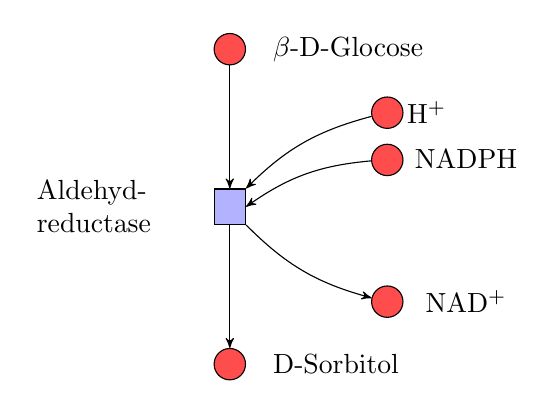
\begin{tikzpicture}[
	block/.style = {draw, fill=blue!30, align=center, anchor=west, minimum height=0.45cm, inner sep=0},
	ball/.style = {circle, draw, fill=red!70, align=center, anchor=north, inner sep=0}]
\node[ball,text width=0.4cm,anchor=base] (glucosepoint) {};
\node[text width=2.9cm,anchor=base,right of=glucosepoint, node distance=2cm] (glucose) {$\beta$-D-Glocose};
\node[block,text width=0.4cm,below of=glucosepoint, node distance=2cm] (aldehydpoint) {}
	edge[<-] (glucosepoint);
\node[text width=2.9cm,left of=aldehydpoint, node distance=1cm] (aldehyd) {Aldehyd-\\reductase};
\node[ball,text width=0.4cm,below of=aldehydpoint, node distance=2cm] (sorbitolpoint) {}
	edge[<-] (aldehydpoint);
\node[text width=2.9cm,anchor=base,right of=sorbitolpoint, node distance=2cm] (glucose) {D-Sorbitol};
\node[ball,text width=0.4cm] at (2,-0.6) {}
	edge[->, bend right=15] (aldehydpoint.north east);
\node at (2.5,-0.8) {H$^+$};
\node[ball,text width=0.4cm] at (2,-1.2) {}
	edge[->, bend right=15] (aldehydpoint.east);
\node at (3,-1.4) {NADPH};
\node[ball,text width=0.4cm] at (2,-3) {}
	edge[<-, bend left=15] (aldehydpoint.south east);
\node at (3,-3.2) {NAD$^+$};
\end{tikzpicture}

\textbf{Filogenia}

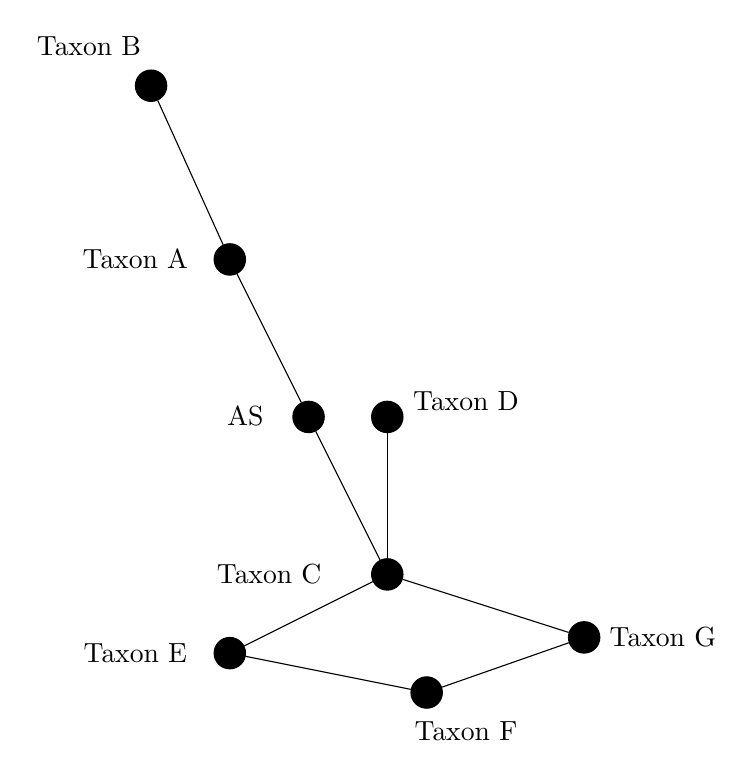
\begin{tikzpicture}[
ball/.style = {circle, draw, fill=black, align=center, anchor=north, inner sep=0}]
\node[ball,text width=0.4cm,anchor=base] (taxonbpoint) {};
\node[text width=2.9cm,anchor=base,above of=taxonbpoint, node distance=0.5cm] {Taxon B};
\node[ball,text width=0.4cm] (taxonapoint) at (1,-2) {}
	edge[-] (taxonbpoint);
\node at (-0.2,-2.2) {Taxon A};
\node[ball,text width=0.4cm] (aspoint) at (2,-4) {}
	edge[-] (taxonapoint);
\node at (1.2,-4.2) {AS};
\node[ball,text width=0.4cm] (taxoncpoint) at (3,-6) {}
	edge[-] (aspoint);
\node at (1.5,-6.2) {Taxon C};
\node[ball,text width=0.4cm] (taxonepoint) at (1,-7) {}
	edge[-] (taxoncpoint);
\node at (-0.2,-7.2) {Taxon E};
\node[ball,text width=0.4cm] (taxonfpoint) at (3.5,-7.5) {}
	edge[-] (taxonepoint);
\node at (4,-8.2) {Taxon F};
\node[ball,text width=0.4cm] (taxongpoint) at (5.5,-6.8) {}
	edge[-] (taxonfpoint)
	edge[-] (taxoncpoint);
\node at (6.5,-7) {Taxon G};
\node[ball,text width=0.4cm] at (3,-4) {}
	edge[-] (taxoncpoint);
\node at (4,-4) {Taxon D};
\end{tikzpicture}

\end{document}